

\tikzset{every picture/.style={line width=0.75pt}} %set default line width to 0.75pt        

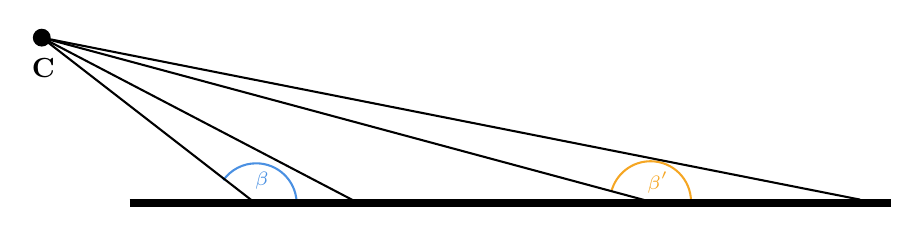
\begin{tikzpicture}[x=0.75pt,y=0.75pt,yscale=-1,xscale=1]
%uncomment if require: \path (0,111); %set diagram left start at 0, and has height of 111

%Shape: Arc [id:dp6607157958124017] 
\draw  [draw opacity=0] (294.74,88.39) .. controls (296.93,80.02) and (304.55,73.85) .. (313.6,73.85) .. controls (324.37,73.85) and (333.1,82.58) .. (333.1,93.35) -- (313.6,93.35) -- cycle ; \draw  [color={rgb, 255:red, 245; green, 166; blue, 35 }  ,draw opacity=1 ] (294.74,88.39) .. controls (296.93,80.02) and (304.55,73.85) .. (313.6,73.85) .. controls (324.37,73.85) and (333.1,82.58) .. (333.1,93.35) ;
%Shape: Arc [id:dp6461315771728425] 
\draw  [draw opacity=0] (107.76,82.98) .. controls (111.29,78.06) and (117.07,74.85) .. (123.6,74.85) .. controls (134.06,74.85) and (142.59,83.08) .. (143.08,93.42) -- (123.6,94.35) -- cycle ; \draw  [color={rgb, 255:red, 74; green, 144; blue, 226 }  ,draw opacity=1 ] (107.76,82.98) .. controls (111.29,78.06) and (117.07,74.85) .. (123.6,74.85) .. controls (134.06,74.85) and (142.59,83.08) .. (143.08,93.42) ;
%Straight Lines [id:da7912546873109455] 
\draw [line width=3]    (62.6,94) -- (429.6,94) ;
%Shape: Circle [id:dp6585955324129855] 
\draw  [draw opacity=0][fill={rgb, 255:red, 0; green, 0; blue, 0 }  ,fill opacity=1 ] (16,14.3) .. controls (16,11.93) and (17.93,10) .. (20.3,10) .. controls (22.67,10) and (24.6,11.93) .. (24.6,14.3) .. controls (24.6,16.67) and (22.67,18.6) .. (20.3,18.6) .. controls (17.93,18.6) and (16,16.67) .. (16,14.3) -- cycle ;
%Straight Lines [id:da6943190688257042] 
\draw    (20.3,14.3) -- (123.6,94.35) ;
%Straight Lines [id:da2008172675955413] 
\draw    (20.3,14.3) -- (171.6,93.35) ;
%Straight Lines [id:da41493445776640725] 
\draw    (20.3,14.3) -- (313.6,93.35) ;
%Straight Lines [id:da4646477074321278] 
\draw    (20.3,14.3) -- (414.6,92.35) ;

% Text Node
\draw (14,23) node [anchor=north west][inner sep=0.75pt]   [align=left] {$\displaystyle \mathbf{C}$};
% Text Node
\draw (121.6,77.35) node [anchor=north west][inner sep=0.75pt]  [font=\scriptsize,color={rgb, 255:red, 74; green, 144; blue, 226 }  ,opacity=1 ] [align=left] {$\displaystyle \beta $};
% Text Node
\draw (310.6,77.35) node [anchor=north west][inner sep=0.75pt]  [font=\scriptsize,color={rgb, 255:red, 245; green, 166; blue, 35 }  ,opacity=1 ] [align=left] {$\displaystyle \beta '$};


\end{tikzpicture}

